%\documentclass[prb,twocolumn,showpacs,aps,floats,floatfix,superscriptaddress]{revtex4}
%\documentclass[prb,showpacs,aps,floats,floatfix,superscriptaddress]{revtex4}
%\documentclass{article}
%\usepackage{epsfig,amsmath,amssymb,array,dcolumn,subfigure,rotating}

\documentclass[onecolumn,letterpaper,amsmath,amssymb,floatfix,aps,superscriptaddress]{revtex4}
%\documentclass[a4paper]{article}
\usepackage{graphicx}% Include figure files
\usepackage{dcolumn}% Align table columns on decimal point
\usepackage{bm}% bold math
\usepackage{epsfig,color}
\usepackage{wrapfig}


\usepackage{epsfig}

\def\ul#1#2{\textstyle{\frac#1#2}}
\def\rot{\operatorname{rot}}
\def\diver{\operatorname{div}}
\def\bnabla{\mbox{\boldmath $\nabla $}}
\def\bepsilon{\mbox{\boldmath $\epsilon $}}

%\renewcommand{\baselinestretch}{1}

\begin{document}

\title{\bf Technical report on the anisotropic cylinder-cylinder interactions at all separations} 

% RUDI, I changed the title here. As far as I understand, this theory cannot work for metallic SWCNTs.

\author{R. Podgornik}
    
\begin{abstract}
I will list all the equations that are needed for numerical implementation of the anisotropic cylinder-cylinder interactions. The code should be
centered around the equations enclosed in frames, Eq. \ref{pars-31a} and Eq. \ref{retardedfinal-a}.
\end{abstract}

\pacs{78.20.Bh, 34.30.-h, 77.22.-d}

\maketitle        

\section{Introduction}


We will write the complete van der Waals -  dispersion interaction free energy between two anisotropic cylinders at all separations, including the retardation effects. 
We start with the Lifshitz theory of van der Waals interactions between two semiinifinte anisotropic uniaxial dielectric layers across a finite layer of dielectric 
function $\epsilon_{m}$ and thickness $\ell$ as worked out by Barash \cite{Barash} - the result of this calculation is the interaction free energy between the two 
layers as a function of their separation $\ell$ and the angle between their principal dielectric anisotropy axes $\theta$: ${\cal G}(\ell,\theta)$. The dielectric 
response of the two dielectrically uniaxial half-spaces is given by the values of their dielectric functions $\overline{\epsilon_{\parallel}}$, parallel and 
$\overline{\epsilon_{\perp}}$, perpendicular to their respective axes.  We shall use $\overline{\epsilon_{1,\parallel}}$ ($\overline{\epsilon_{1,\perp}}$) and 
$\overline{\epsilon_{2,\parallel}}$ ($\overline{\epsilon_{2,\perp}}$) for the left and right half-spaces, respectively. Note also that in the theory of van der 
Waals interactions \cite{Parsegian,Ninham} all the dielectric response functions are evaluated at imaginary frequencies, 
thus $\epsilon_{\parallel,\perp} = \epsilon_{\parallel,\perp}(i \omega)$. $\epsilon_{\parallel,\perp}(i \omega)$ is referred to as the London - van der Waals 
transform of the response function $\epsilon_{\parallel,\perp}(\omega)$ and is given by the Kramers - Kronig relations. It is strictly a real, monotonically 
decaying function of $\omega$. 

\begin{figure}
\centerline{\includegraphics[width=8cm]{./140220_cyl-cyl/sketch.pdf}}
%\epsfig {file=sketch.pdf,width=5cm}}
\caption{A sketch of the system of interest (the two cylinders). The quantities describing the geometry of the system are 
denoted, together with the logitudinal and transverse directions of cylinder in the left half-space (1). The skew angle $\theta$ is about an axis normal to the planar boundary defining the limits of each half-space.
}
\label{fig:sketch}
\end{figure}


From the interaction free energy between two half-spaces one can extract the interaction between two cylinders (see Fig. \ref{fig:sketch}) by assuming that the two half-spaces are 
dilute assemblies of anisotropic cylinders. One should keep in mind, however, that the cylinder dielectric response is isotropic in the plane perpendicular 
to the cylinder axis - we call this the transverse dielectric response. The difference between the transverse response and the response in the direction parallel 
to the cylinder axis (longitudinal response) constitutes the dielectric anisotropy of the problem. The derivation closely follows the arguments of Pitaevskii 
for evaluating the interactions between isotropic impurity 
atoms in a homogeneous fluid \cite{Pitaevskii}. 
We assume that the two anisotropic half-spaces are composed of anisotropic cylinders of radii $R_1$ and $R_2$ at volume fractions $v_1$ and $v_2$, with 
${\epsilon^{c}}_{1,\perp}$ (${\epsilon^{c}}_{2,\perp}$) and ${\epsilon^{c}}_{1,\parallel}$ (${\epsilon^{c}}_{2,\parallel}$) as the 
transverse and longitudinal dielectric response functions of the cylinder materials. We then expand ${\cal G}(\ell,\theta)$ for two half-spaces 
as a series in $v_1$ and $v_2$ and evaluate the coefficient multiplying the $v_1 v_2$ term. The volume 
fractions $v_1$ and $v_2$ scale with the area density of the cylinders ($N_1, N_2$) in the direction of their long axes as $v_1 = N_1~\pi R_1^{2}$ ($v_2 = N_2~\pi R_2^{2}$). It then follows \cite{Parsegian} that the interaction free energy between two cylinders, $G(\ell,\theta)$, whose axes are contained within the two parallel boundaries 
at a separation $\ell$, but skewed at an angle $\theta$ (see Fig. \ref{fig:sketch}) is given by 
\begin{equation}
\frac{d^{2}{\cal G}(\ell,\theta)}{d\ell^{2}}= N_1 N_2\sin{\theta}~G(\ell,\theta).
\label{form1}
\end{equation}
Conversely, the interaction free energy {\sl per unit length}, $g(\ell)$, between two parallel cylinders is given by the Abel transform (see e.g. Ref. \onlinecite{Parsegian}, pp 233-235)
\begin{equation}
\frac{d^{2}{\cal G}(\ell,\theta=0)}{d\ell^{2}}=N_1 N_2\int_{-\infty}^{+\infty}g(\sqrt{\ell^{2}+y^{2}})~dy.
\label{form2}
\end{equation}
In both cases we expand ${\cal G}(\ell,\theta)$ to find the coefficient next to $v_1 v_2$ (or equivalently $N_1 N_2$), take the second derivative with respect to $\ell$, then use Eqs. \ref{form1} and \ref{form2} in order to obtain the appropriate pair interaction free energy between cylinders. Note that such an expansion is possible only if the dielectric response at all frequencies is bounded. In the case of an ideal metal Drude-like dielectric response this expansion is not feasible and our method can not be transplanted to that case automatically.

The closest attempt in the literature to evaluate the interaction between two cylinders at all separations comes from Barash and Kyasov \cite{Barash89}.  Where this approach can be compared with the one presented here, {\sl i.e.} for two parallel isotropic cylinders, the results for the interaction free energy between parallel cylinders coincide completely. The results described below were published in A. \v Siber, R. F. Rajter, R. H. French, W. Y. Ching, V. A. Parsegian, and R. Podgornik: {\sl Dispersion interactions between optically anisotropic cylinders at all separations: Retardation effects for insulating and semiconducting single-wall carbon nanotubes}, PHYSICAL REVIEW B 80, 165414 (2009).

\section{Derivation}

We use the Pitaevskii {\sl ansatz} in order to extract the interactions between two infinite anisotropic cylinders at all separations and angles from the interaction between 
two semi-infinite half-spaces of anisotropic uniaxial dielectric material. We start with the fully retarded van der Waals - dispersion interactions between two semiinfinite anisotropic 
dielectric slabs \cite{Barash}. The full interaction form is quite involved, but it has a simple limit if the two semiinfinite slabs, ${\cal L}$ and ${\cal R}$, separated by an isotropic medium of thickness $\ell$, are composed of rarefied material. 

In order to get the interaction free energy between two anisotropic cylinders we assume that both semi-infinite substrates (half-spaces), ${\cal L}$ ($1$) and ${\cal R}$ ($2$), are 
composite materials made of oriented anisotropic cylinders at volume fractions $v_1$ and $v_2$, with ${\epsilon^{c}}_{1,\perp}$ (${\epsilon^{c}}_{2,\perp}$) 
and ${\epsilon^{c}}_{1,\parallel}$ (${\epsilon^{c}}_{2,\parallel}$) as the transverse and longitudinal
dielectric response functions of the cylinder materials. For the semi-infinite composite medium of oriented anisotropic cylinders with local hexagonal  packing symmetry, so that the corresponding cylinder volume fraction is $v$, the anisotropic bulk dielectric response function can be derived in the
form (see Ref. \onlinecite{Parsegian}, p.318) 
\begin{equation}
\overline{\epsilon_{\parallel}}=\epsilon_{m}\left(1+v\Delta_{\parallel}\right),\qquad\overline{\epsilon_{\perp}}=\epsilon_{m}\left(1+\frac{2v\Delta_{\perp}}{1-v\Delta_{\perp}}\right),\label{eq:v_dependance}
\end{equation}
where the relative anisotropy measures in the parallel and perpendicular direction are given by
\begin{equation}
\Delta_{\perp}=\frac{{\epsilon^{c}}_{\perp}-\epsilon_{m}}{{\epsilon^{c}}_{\perp}+\epsilon_{m}}\qquad\Delta_{\parallel}=\frac{{\epsilon^{c}}_{\parallel}-\epsilon_{m}}{\epsilon_{m}}.
\label{anisoind}
\end{equation}

%%%%%%%%%EPS2%%%%%%%%%%%%%%%%%%%%%%%%%%%%%%%%%%%%%%%%%%%%%%%%%%%%%%%%%%%%%%%%%%
\begin{figure}
\centerline{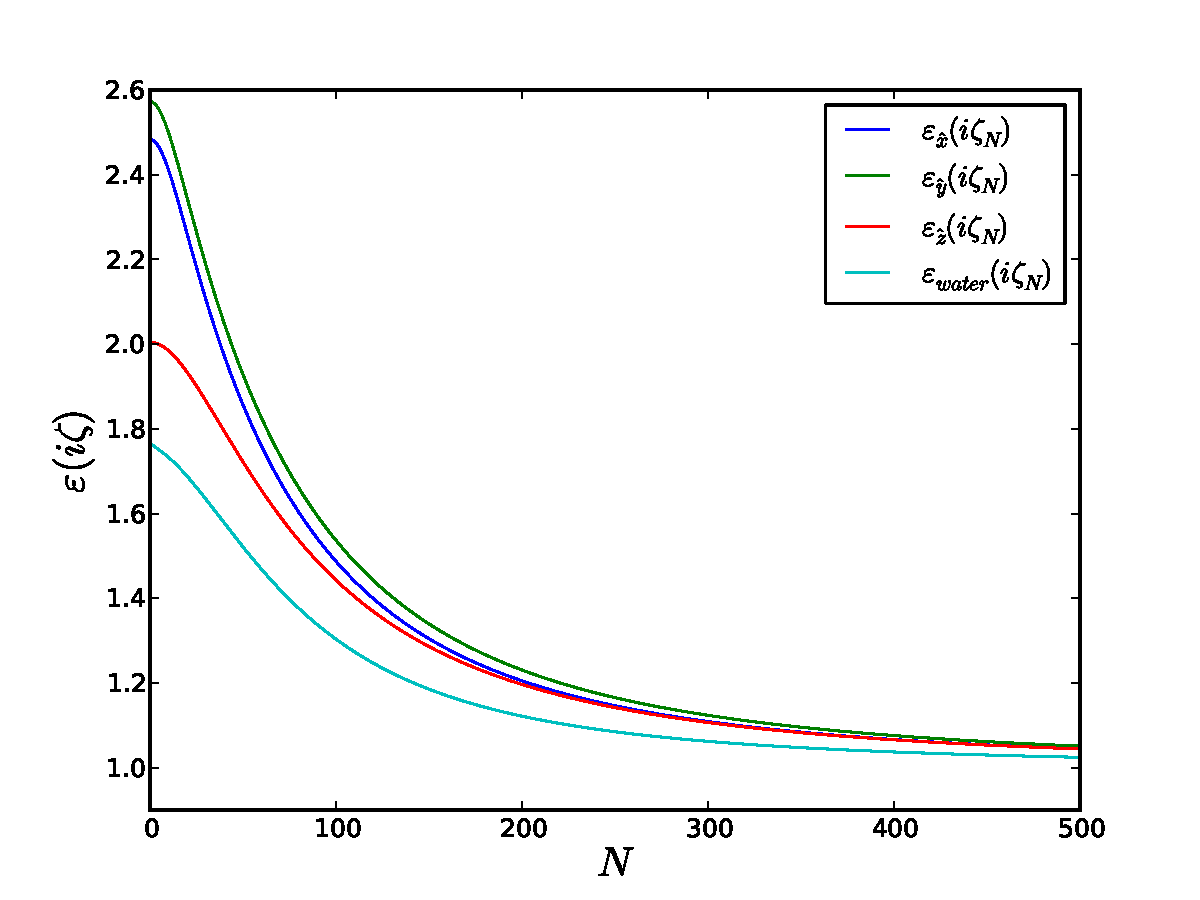
\includegraphics[width=8cm]{./140220_cyl-cyl/eiz.pdf}}
\caption{\label{fig:1} Anisotropic response functions for CG-10 DNA and water. The DNA response functions in the x and y directions were used as perpendicular and parallel inputs, respectively.  CG-10 and water eps2 data was provided by Dan Dryden. CG-10 data scales Wai-Yim's calculations by 4.94 and is assumed to include Na (more info in Dan Dryden email sent to us on Nov. 8, 2013).  Water data was built from lorentz oscillators R.H.French,J.Amer.Ceram Soc.,83,9,2117-46(2000), H.D.Ackler, et al,J.Coll.Interface Sci.179,46. }
\end{figure}

In our case, this holds for both ${\cal L}$ and ${\cal R}$ half-spaces with the appropriate volume fractions and dielectric responses. $\epsilon_{m}$ is the dielectric function of the 
isotropic medium between the cylinders as well as between regions ${\cal L}$ and ${\cal R}$. We assume in what follows that all the response functions are bounded and finite.
 
The formulae in Eqs. \ref{form1},\ref{form2} connect the interaction free energy of two semiinifinite half spaces with the interaction free energy between two cylinders either 
parallel or skewed at a finite angle $\theta$. The Barash result \cite{Barash} for the complete retarded form of the interactions between two uniaxial media, ${\cal G}(\ell,\theta)$, 
is quite complicated (note also a typo that propagated starting from the original version of the calculation \cite{erratum} and was first noted in Ref. \onlinecite{philbin}) but can be straightforwardly expanded to second order 
in $N$ (a term proportional to $v_1 v_2$) for the dielectric response functions of the form Eq. \ref{eq:v_dependance}, yielding the following result
\begin{equation}
\frac{d^{2}{\cal G}(\ell,\theta)}{d\ell^{2}} = \frac{k_BT}{2\pi} {\sum_{n=0}^{\infty}}' \int_0^{\infty} Q dQ \frac{d^{2}f(\ell,\theta)}{d\ell^{2}}.
\end{equation}
In the above equation, $n$ represent the (thermal) Matsubara indices, the prime on the summation means  that the weight of the $n=0$ term is 1/2 (see Refs. \onlinecite{Parsegian,Barash89} for details). The second derivative of the function $f(\ell,\theta)$ can be obtained explicitly 
in terms of the ratios between the relative anisotropy measures (Eq. \ref{anisoind}) defined as 
\begin{equation}
a = \frac{2 \Delta_{\perp}}{\Delta_{\parallel}} = 2 \frac{({\epsilon^{c}}_{\perp}-\epsilon_{m}) \epsilon_{m}}{({\epsilon^{c}}_{\perp}+\epsilon_{m}) ({\epsilon^{c}}_{\parallel}-\epsilon_{m})}
\label{eq:adef}
\end{equation}
and is obviously frequency dependent. Parameters $a_1$ and $a_2$ can be thought of as a specific measure of the anisotropy of the cylinders in the left and right half-spaces when 
compared with the isotropic bathing medium $m$. Note that they vanish when the transverse dielectric response of the cylinder material equals the medium response. 
The explicit form of the second derivative of $f(\ell,\theta)$ now follows as 

\begin{widetext}
\begin{eqnarray}
\frac{d^{2}f(\ell,\theta)}{d\ell^{2}} &=& - \frac{v_1 v_2 \Delta_{1,\parallel} \Delta_{2,\parallel}}{32} 
\frac{e^{-2 \ell \sqrt{Q^{2} + \epsilon_m \frac{\omega_n^{2}}{c^{2}}}}}{(Q^{2} + \epsilon_m \frac{\omega_n^{2}}{c^{2}})} \nonumber \\
& &
\left\{ 2 \left[ (1+3a_1)(1+3a_2) Q^{4} + 2 (1+2a_1+2a_2+3a_1a_2) Q^{2} \epsilon_m \frac{\omega_n^{2}}{c^{2}} + 2(1+a_1)(1+a_2) {\epsilon_m}^{2} \frac{\omega_n^{4}}{c^{4}}\right] \right. + \nonumber\\
& & \left. ~~~~~~~~~~~~~~~~~~~~~~~~~~~~~~~~~~~~~~~~~~~~~~~~~~~~ + (1-a_1)(1-a_2)\left( Q^{2} + 2 \epsilon_m \frac{\omega_n^{2}}{c^{2}} \right)^2 \cos 2\theta \right \}.
\label{eq:d2f}
\end{eqnarray}
\end{widetext}
Here $R_1$ and $R_2$ are the cylinder radii, assumed to be the smallest lengths in the problem \cite{Barash89}. The frequency dependence of the dielectric functions is in 
$\epsilon_m(i \omega_n)$, ${\epsilon^{c}}_{\perp}(i \omega_n)$ and ${\epsilon^{c}}_{\parallel}(i \omega_n)$, and therefore also $a = a(i \omega_n)$. The frequencies 
in the Matsubara summation are $\omega_n = 2\pi~\frac{k_BT}{\hbar} n$. Note that Eq. \ref{eq:d2f} is symmetric with respect to 1 and 2 indices (left and right 
half-spaces), as it should be.

This is as far as a general theory can go. We must now deal separately with the cases of skewed and parallel cylinders, since the connection 
between $\frac{d^{2}{\cal G}(\ell,\theta)}{d\ell^{2}}$ and the effective pair interaction between cylinders is different for the two cases, 
see Eqs. \ref{form1},\ref{form2}. We first analyze the case of skewed cylinders.

\section{Skewed cylinders}

\subsection{Skewed cylinders - full result}

We use  Eq. \ref{form1} to obtain the interaction free energy between two skewed cylinders:
\begin{equation}
G(\ell,\theta) = - \frac{k_BT}{64 \pi} \frac{ \pi^2 R_1^{2} R_2^{2} }{\ell^{4} \sin{\theta}} {\sum_{n=0}^{\infty}}' \Delta_{1,\parallel} \Delta_{2,\parallel} \int_0^{\infty}  u du ~\frac{e^{- 2 \sqrt{u^{2} + p_n^{2}}}}{(u^{2} + p_n^{2})}  g(a_1, a_2, u, p_n, \theta),
\label{pars-3}
\end{equation}
where $u = Q \ell$,  
\begin{widetext}
\begin{eqnarray}
g(a_1, a_2, u, p_n, \theta) &=&  2 \left[ (1+3a_1)(1+3a_2) u^{4} + 2(1+2a_1+2a_2+3a_1a_2) u^{2}p_n^{2}  + 2(1+a_1)(1+a_2) p_n^{4}\right] + \nonumber \\ 
& & ~~~~~~~~~~~~~~~~~~~~~~~~~~~~~~~~~~~~~~~~~ + (1-a_1)(1-a_2)(u^{2} + 2 p_n^{2})^2 \cos 2\theta
\end{eqnarray}
\end{widetext}
and $p_n^{2}(\ell) =  \epsilon_m(i \omega_n) \frac{\omega_n^{2}}{c^{2}} \ell^{2}$. Another change of variables with $u = p_n t$, yields 
\begin{equation}
G(\ell,\theta) = - \frac{k_BT}{64 \pi} \frac{ \pi^2 R_1^{2} R_2^{2} }{\ell^{4} \sin{\theta}} {\sum_{n=0}^{\infty}}' \Delta_{1,\parallel} \Delta_{2,\parallel} ~p_n^{4} ~\int_0^{\infty} t dt ~\frac{e^{- 2 p_n \sqrt{t^{2} + 1}}}{(t^{2} + 1)} \tilde g(t, a_1(i \omega_n), a_2(i \omega_n), \theta),
\label{pars-31}
\end{equation}
with
\begin{widetext}
\begin{eqnarray}
\tilde g(t, a_1, a_2, \theta) &=& 2 \left[ (1+3a_1)(1+3a_2) t^{4} + 2 (1+2a_1+2a_2+3a_1a_2) t^{2}  + 2(1+a_1)(1+a_2)\right] + \nonumber \\
& & ~~~~~~~~~~~~~~~~~~~~~~~~~~~~~~~~~~~~~~~~~ + (1-a_1)(1-a_2)(t^{2} + 2)^2 \cos 2\theta.
\label{pars-31-g}
\end{eqnarray}
\end{widetext}
This is the final result for the cylinder-cylinder interaction at all angles when the radii of the cylinders are the smallest lengths in the system. It includes retardation and the full angular dependence. Some simple limits can be obtained form this general expression.

%%%%%%%%%Full_skew_G_vs_l,theta%%%%%%%%%%%%%%%%%%%%%%%%%%%%%%%%%%%%%%%%%%%%%%%%
\begin{figure*}[t!]
\begin{center}
\begin{minipage}[b]{0.40\textwidth}
\begin{center}
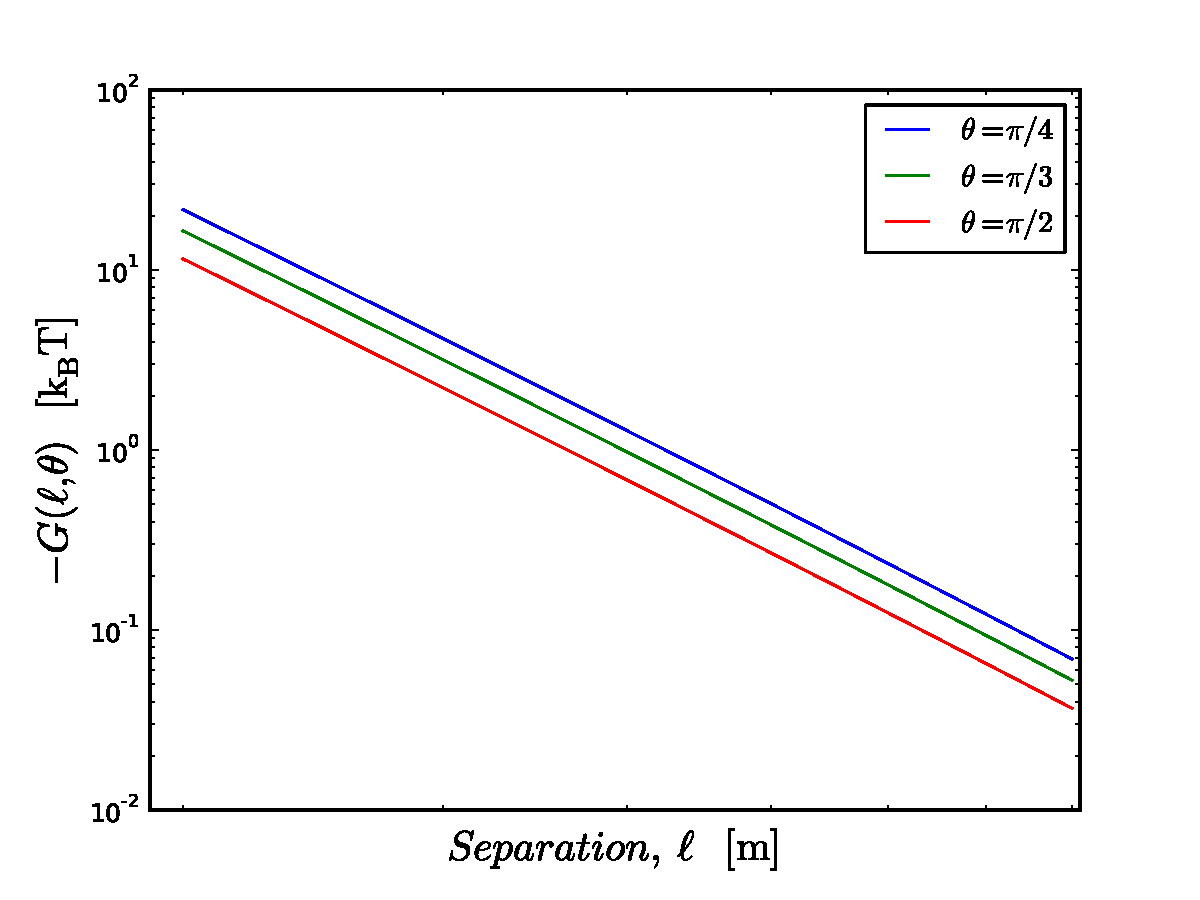
\includegraphics[width=1.2\textwidth]{./140220_cyl-cyl/Full_skew_G_vs_l.pdf} (a)
\end{center}
\end{minipage}
\hskip 43pt
\begin{minipage}[b]{0.40\textwidth}
\begin{center}
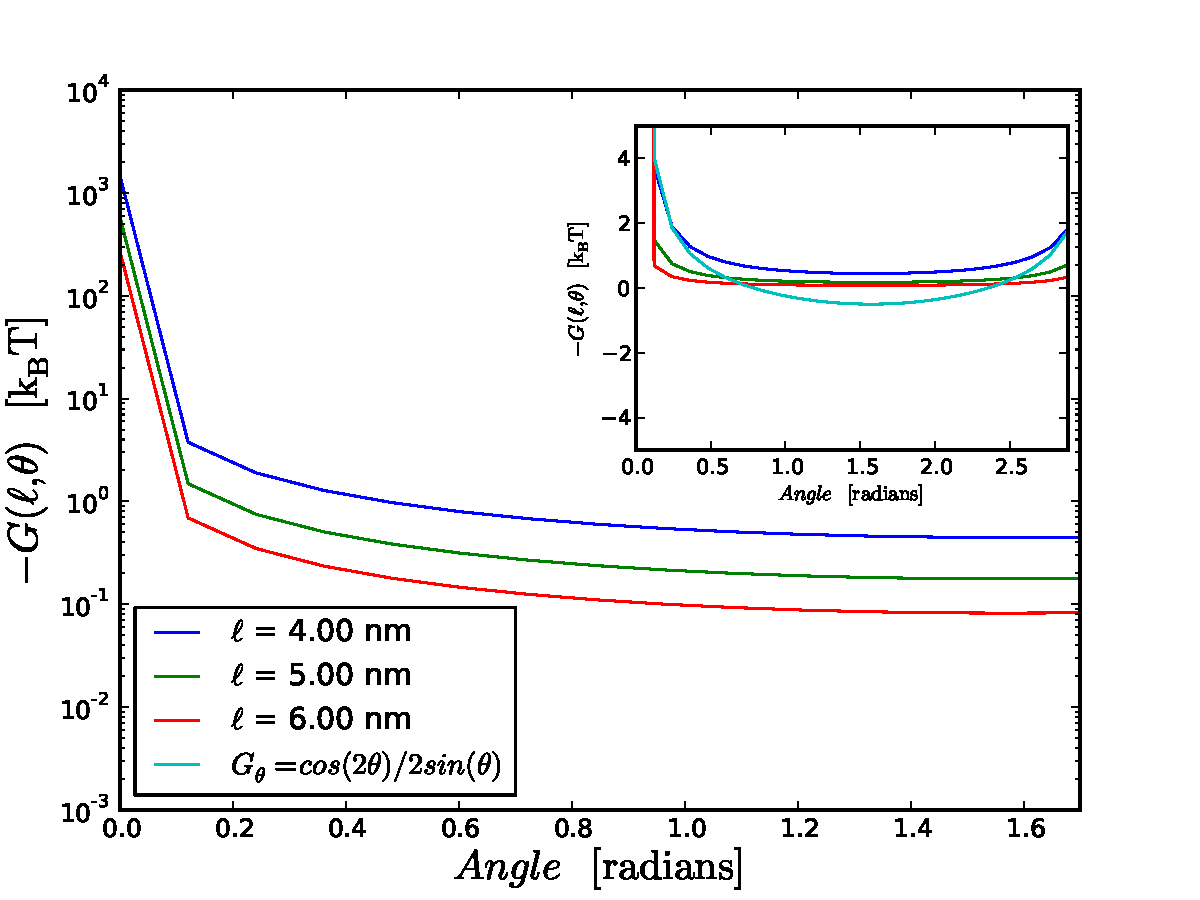
\includegraphics[width=1.2\textwidth]{./140220_cyl-cyl/Full_skew_G_vs_theta.pdf} (b)
\end{center}
\end{minipage}
\caption{Full result using Eqs.\ref{pars-31},\ref{pars-31-g} (a) Interaction free energy between two cylinders (CG-10 DNA) with radii of 1 nm in water plotted as a function of separation from 2 to 8 nm, for three values of mutual angle. (b) Interaction as a function of mutual angle (0 radians to $\pi/2$ radians) at three values of separation.  The inset shows the periodic behavior of $G(\ell,\theta)$ over an interval $\pi$ for three values of separation. The cyan curve shows the behavior of the theta dependance of $G$  }
\label{fiddle1}
\end{center}
\end{figure*} 

We now transform this result into a form that is suitable for computation and numerical implementation. First we rewrite Eq. \ref{pars-31} as
\begin{equation}
  \fbox{
    $\displaystyle{
G(\ell,\theta) = - \frac{ (\pi R_1^{2})(\pi R_2^{2}) }{2 \pi~\ell^{4} \sin{\theta}} \left( {\cal A}^{(0)}(\ell) + {\cal A}^{(2)}(\ell) \cos 2\theta \right) ,}$}
\label{pars-31a}
\end{equation}
The $(\ell)$ dependence of the Hamaker coefficients $\cal A$ is a consequence of $(\ell)$ dependence of $p_n^{2}(\ell) =  \epsilon_m(i \omega_n) \frac{\omega_n^{2}}{c^{2}} \ell^{2}$. Above we defined
\begin{widetext}
\begin{equation}
{\cal A}^{(0)}(\ell) = \frac{k_BT}{32}  {\sum_{n=0}^{\infty}}' \Delta_{1,\parallel} \Delta_{2,\parallel} ~p_n^{4}(\ell) ~\int_0^{\infty} t dt ~\frac{e^{- 2 p_n(\ell) \sqrt{t^{2} + 1}}}{(t^{2} + 1)} \tilde g^{(0)}(t, a_1(i \omega_n), a_2(i \omega_n))
\label{eq:a0}
\end{equation}
\end{widetext}
with
\begin{equation}
\tilde g^{(0)}(t, a_1(i \omega_n), a_2(i \omega_n)) = 2 \left[ (1+3a_1)(1+3a_2) t^{4} + 2 (1+2a_1+2a_2+3a_1a_2) t^{2}  + 2(1+a_1)(1+a_2)\right]
\end{equation}
and
\begin{widetext}
\begin{equation}
{\cal A}^{(2)}(\ell) = \frac{k_BT}{32}  {\sum_{n=0}^{\infty}}' \Delta_{1,\parallel} \Delta_{2,\parallel} ~p_n^{4}(\ell) ~\int_0^{\infty} t dt ~\frac{e^{- 2 p_n(\ell) \sqrt{t^{2} + 1}}}{(t^{2} + 1)} \tilde g^{(2)}(t, a_1(i \omega_n), a_2(i \omega_n), \theta)
\end{equation}
\end{widetext}
with
\begin{equation}<C-LeftRelease>
\tilde g^{(0)}(t, a_1(i \omega_n), a_2(i \omega_n), \theta) = (1-a_1)(1-a_2)(t^{2} + 2)^2
\label{befgqw}
\end{equation}

The numerical implementation should be for Eqs. \ref{pars-31a}-\ref{befgqw}. For $a_{1,2}$ one invokes the previous definition Eq. \ref{eq:adef}
\begin{equation}
a_{1,2}(i \omega_n) = \frac{2 \Delta_{\perp}^{(1,2)}(i \omega_n)}{\Delta_{\parallel}^{(1,2)}(i \omega_n)} = 2 \frac{({{\epsilon^{c}}_{\perp}}^{(1,2)}(i \omega_n) -\epsilon_{m}(i \omega_n)) \epsilon_{m}(i \omega_n)}{({{\epsilon^{c}}_{\perp}}^{(1,2)}(i \omega_n)+\epsilon_{m}(i \omega_n)) ({{\epsilon^{c}}_{\parallel}}^{(1,2)}(i \omega_n) -\epsilon_{m}(i \omega_n))}
\label{eq:adef}
\end{equation}
where ${{\epsilon^{c}}_{\perp}}^{(1,2)}$, ${{\epsilon^{c}}_{\parallel}}^{(1,2)}$ are the perpendicular, parallel components of the dielectric response functions of the two cylinders and $\epsilon_{m}$ is the same for the medium in between. All these quantities are of course frequency dependent. The $n$ summation is over the Matsubara frequencies, $\zeta_n = 2\pi n k_BT/\hbar$, where $n$ is an integer and the $n=0$ term is counted with a weight $1/2$. At room temperature the Matsubara frequencies are a multiple of $\rm 2.4 \times 10^{14}~s^{-1}$.

%%%%%%%%%%%%%%%%%%%%%%%%%%%%%%%%%%%%%%%%%%%%%%%%%%%%%%%%%%%%%%%%%%%%%%%%%%%%%%%
%AIZ and A0,A2
\begin{figure*}%[t!]
\begin{center}
\begin{minipage}[b]{0.40\textwidth}
\begin{center}
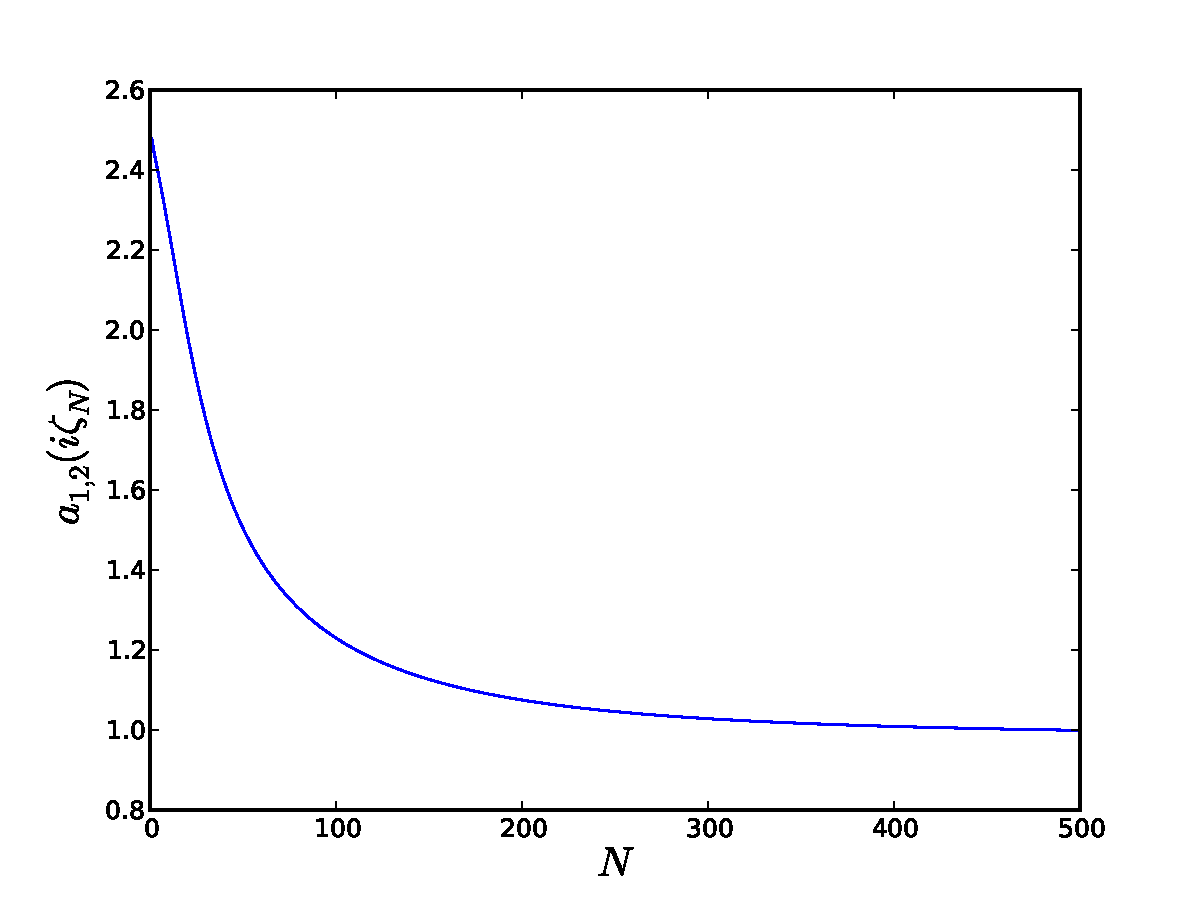
\includegraphics[width=1.2\textwidth]{./140220_cyl-cyl/aiz.pdf} (a)
\end{center}
\end{minipage}
\hskip 43pt
\begin{minipage}[b]{0.40\textwidth}
\begin{center}
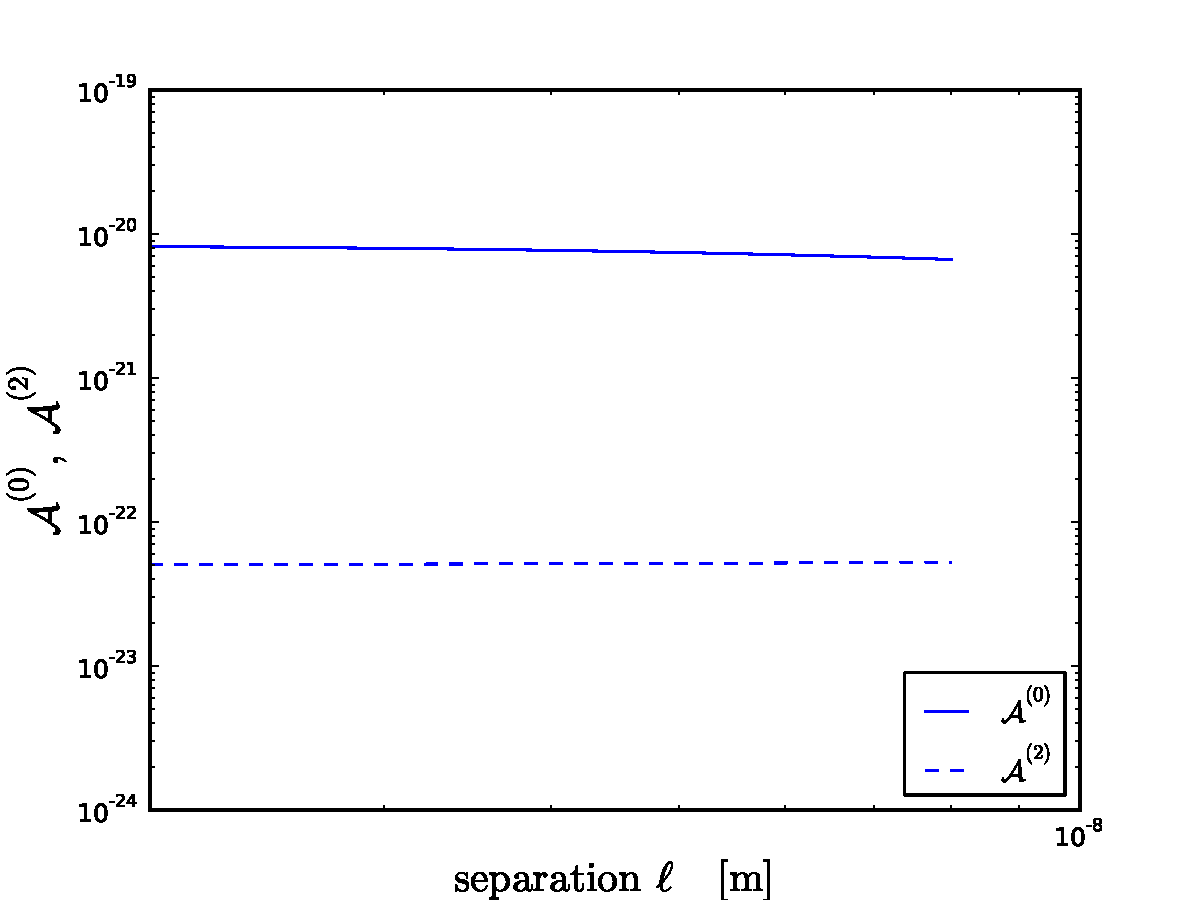
\includegraphics[width=1.2\textwidth]{./140220_cyl-cyl/Full_skew_A0_A2.pdf} (b)
\end{center}
\end{minipage}
\caption{(a) Anistropy metric $a_{1,2}(i\zeta_n)$ using Eq.\ref{eq:adef}, compares the anisotropy of the  cylinders (DNA) to their intervening material, water for the terms contruting to the Matsubara sum. (b) Hamaker coeffcients ${\cal A}^{(0)}(\ell)$ (solid line) and ${\cal A}^{(2)}(\ell)$ (dashed line) calculated using fully retarded formulation, Eqs.\ref{eq:a0}-\ref{befgqw}.}
\label{fiddle1}
\end{center}
\end{figure*} 

\subsection{Skewed cylinders - non-retarded result}

The  non-retarded limit where $c \longrightarrow \infty$, has already been explored in Ref. \onlinecite{rick2}. There $p_n \longrightarrow 0$ for all $n$ and we obtain from Eq. \ref{pars-3}
\begin{widetext}
\begin{eqnarray}
G(\ell,\theta; c \longrightarrow \infty) &=& - \frac{k_BT}{64 \pi} \frac{\pi^{2} R_1^{2} R_2^{2} }{\ell^{4} \sin{\theta}} {\sum_{n=0}^{\infty}}' \Delta_{1,\parallel} \Delta_{2,\parallel}
\int_0^{\infty} u^{3} du ~{e^{- 2 u}} \left[ 2 (1+3a_1)(1+3a_2) + (1-a_1)(1-a_2)  \cos 2\theta \right] = \nonumber\\
&=& - \frac{k_BT}{64 \pi} \frac{\pi^{2} R_1^{2} R_2^{2}}{\ell^{4} \sin{\theta}} {\sum_{n=0}^{\infty}}' \Delta_{1,\parallel} \Delta_{2,\parallel}
 \frac{3}{8}\left[ 2 (1+3a_1) (1+3a_2) + (1-a_1) (1-a_2)  \cos 2\theta \right].
\label{pars-4}
\end{eqnarray}
\end{widetext}
This formula could also be obtained directly from Eq. \ref{pars-31} taking into account that in the $t$ integration only the terms with large $t$ contribute to the final integral. Expanding the whole integrand for large $t$ returns us to Eq. \ref{pars-4}. The $n = 0$ term of this formula for two identical cylinders corresponds to classical dipolar fluctuation forces as analyzed in \onlinecite{parscylinders}.

%%%%%%%%%%%%%%%%%%%%%%%%%%%%%%%%%%%%%%%%%%%%%%%%%%%%%%%%%%%%%%%%%%%%%%%%%%%%%%%
%NR_skew_G_vs_l,theta
\begin{figure*}[t!]
\begin{center}
\begin{minipage}[b]{0.40\textwidth}
\begin{center}
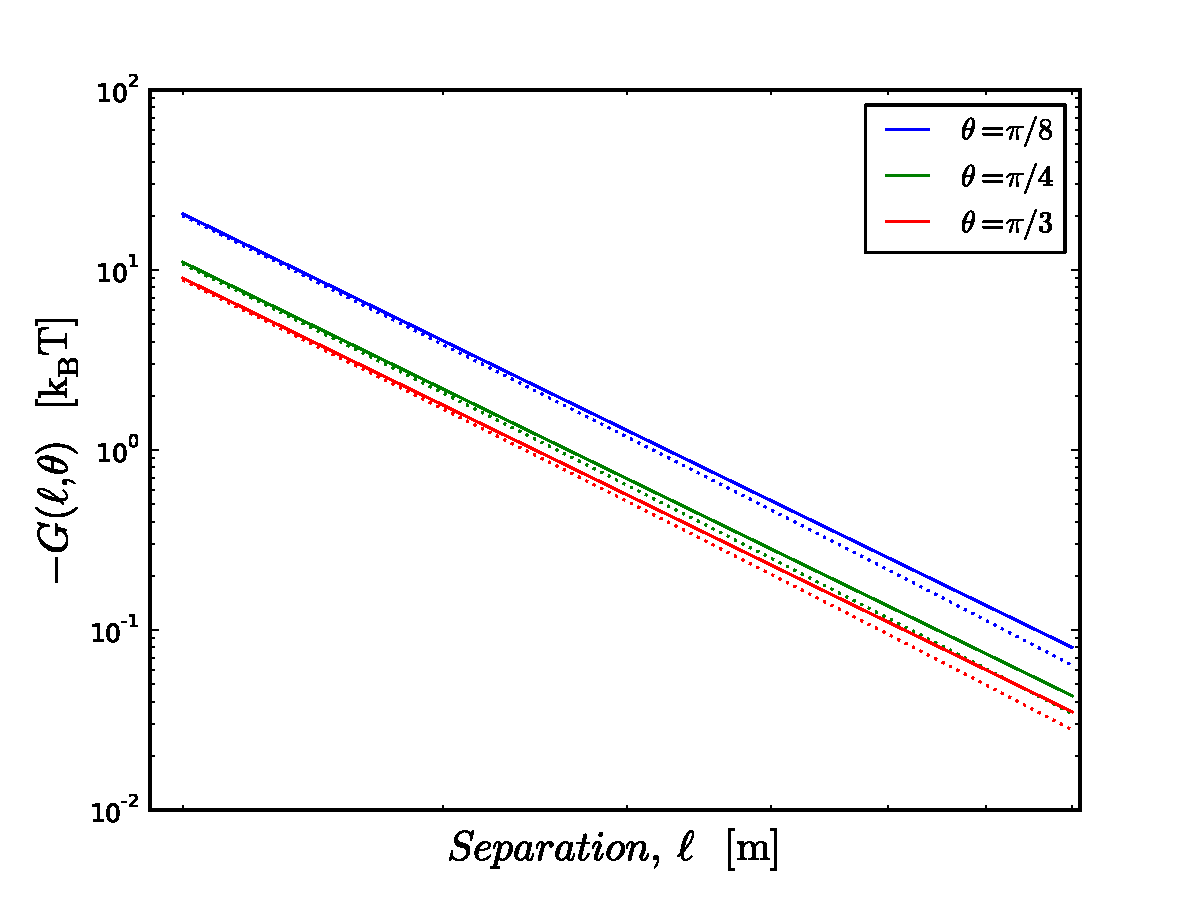
\includegraphics[width=1.2\textwidth]{./140220_cyl-cyl/Compare_full_nonret_G_vs_l.pdf} (a)
\end{center}
\end{minipage}
\hskip 43pt
\begin{minipage}[b]{0.40\textwidth}
\begin{center}
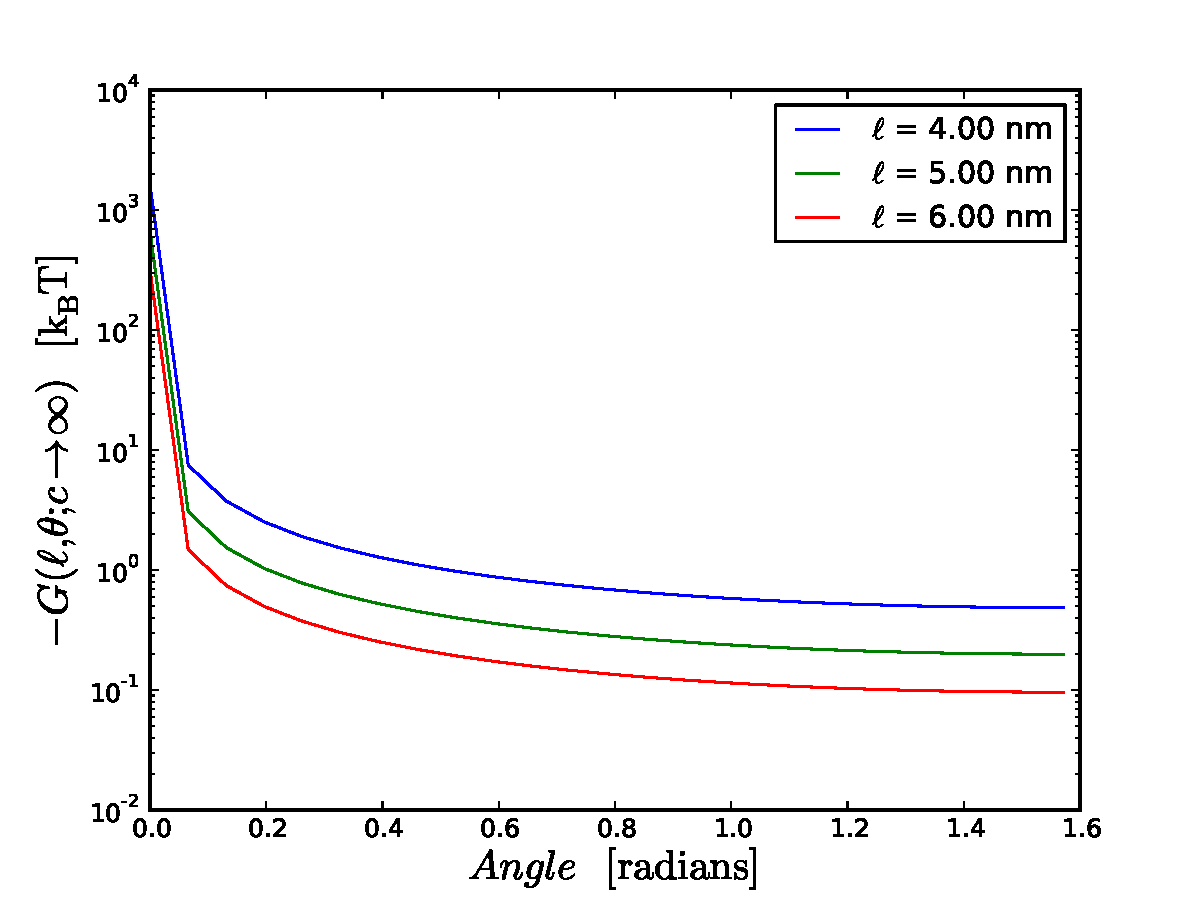
\includegraphics[width=1.2\textwidth]{./140220_cyl-cyl/Nonret_skew_G_vs_theta.pdf} (b)
\end{center}
\end{minipage}
\caption{Non-retarded result using Eq.\ref{pars-4} (a) The nonretarded interaction free energy between two cylinders is shown as solid lines as a function of separation (2 nm to 8 nm) for three values of mutual angle. Dashed lines show retarded calculations for the same parameter values. (b) Interaction as a function of mutual angle from 0 to $\pi/2$ for three values of separation.}
%\label{}
\end{center}
\end{figure*} 

\subsection{Skewed cylinders - low temperature result}

At low temperatures, when the summation over the Matsubara frequencies can be turned into an integral over $n$ with $dn = \hbar/(2\pi ~k_BT) d\omega$, the corresponding interaction free energy is  
\begin{widetext}
\begin{equation}
G(\ell,\theta) = - \frac{\hbar}{128 \pi^2} \frac{\pi^2 R_1^{2} R_2^{2}}{c^{4} \sin{\theta}} \int_{0}^{\infty}\!\!\! d\omega~ \omega^{4}  
\Delta_{1,\parallel}(i\omega) \Delta_{2,\parallel}(i\omega) \epsilon_m(i\omega)^2\!\!\!\int_0^{\infty}\!\!\! t dt ~\frac{e^{- 2 \sqrt{\epsilon_m(i \omega)} 
\frac{\omega}{c} \ell \sqrt{t^{2} + 1}}}{(t^{2} + 1)} \tilde g(t, a_1(i \omega), a_1(i \omega), \theta).
\label{pars-32}
\end{equation}
\end{widetext}
We now rework this equation to obtain the retarded result for the interaction between two semiconducting cylinders. Note here that we can not derive the Casimir limit properly  
as our formulation is not valid for nominally infinite zero-frequency (Drude-like) dielectric response. For that case see  Ref. \onlinecite{Barash89}. First instead of  variable $\omega$, we introduce 
$x = \frac{\ell}{c} \sqrt{t^2 + 1} ~\omega$. Then, following closely the arguments in Ref. \onlinecite{LL} we obtain  the interaction free energy in the form
\begin{widetext}
\begin{equation}
G(\ell,\theta) = - \frac{\hbar c}{128 \pi^2} \frac{\pi^2 R_1^{2} R_2^{2}} { \ell^5\sin{\theta}} \epsilon_m(0)^2 \Delta_{1,\parallel}(0) \Delta_{2,\parallel}(0) 
\int_{0}^{\infty}\!\!\! dx~ x^{4}   \!\!\!\int_0^{\infty}\!\!\! t dt ~\frac{e^{- 2 \sqrt{\epsilon_m(0)}x}}{(t^{2} + 1)^{7/2}}~ \tilde g(t, a_1(0), a_2(0), \theta).
\label{pars-33}
\end{equation}
\end{widetext}
Here $\epsilon_m(0)$ and $a_1(0), a_2(0)$ denote the static, {\sl i.e.} zero frequency, values of the corresponding functions. 
Obviously in this regime the interaction free energy decays faster with separation, being a reflection of the retardation. All the frequency 
dependence of the material properties is reduced to the static response in this limit, just as in the general Lifshitz analysis \cite{LL}.

\section{Parallel cylinders}

\subsection{Parallel cylinders - full result}

The analysis here is somewhat more complicated because the pair interaction energy between the cylinders involves the inverse Abel transform \cite{Abel}. We start with
\begin{equation}
\frac{d^{2}{\cal G}(\ell,\theta = 0)}{d\ell^{2}} = \frac{k_BT}{2\pi} {\sum_{n=0}^{\infty}}' \int_0^{\infty} Q dQ \frac{d^{2}f(\ell,\theta = 0)}{d\ell^{2}},
\label{equnew1}
\end{equation}
where  
\begin{widetext}
\begin{eqnarray}
\frac{d^{2}f(\ell,\theta = 0)}{d\ell^{2}} &=& - \frac{v_1 v_2 \Delta_{1,\parallel} \Delta_{2,\parallel}}{32} 
\frac{e^{-2 \ell \sqrt{Q^{2} + \epsilon_m \frac{\omega_n^{2}}{c^{2}}}}}{(Q^{2} + \epsilon_m \frac{\omega_n^{2}}{c^{2}})} \nonumber \\
& & \left \{ 2 \left [ (1+3a_1)(1+3a_2) Q^{4} + 2 (1+2a_1+2a_2+3a_1a_2) Q^{2} \epsilon_m \frac{\omega_n^{2}}{c^{2}} + 2(1+a_1)(1+a_2) 
{\epsilon_m}^{2} \frac{\omega_n^{4}}{c^{4}}\right] \right. + \nonumber\\
& &~~~~~~~~~~~~~~~~~~~~~~~~~~~~~~~~~~~~~~~~~~~~~ +  \left. (1-a_1)(1-a_2)(Q^{2} + 2 \epsilon_m \frac{\omega_n^{2}}{c^{2}})^2 \right \},
\label{equnew2}
\end{eqnarray}
\end{widetext}
and again $v_1 = N~\pi R_1^{2}$ ($v_2 = N~\pi R_2^{2}$) and $a = \frac{2 \Delta_{\perp}}{\Delta_{\parallel}}$. We continue by introducing the Abel transform and its properties. Namely, if we define
\begin{equation}
\int_{-\infty}^{+\infty}g(\sqrt{\ell^{2}+y^{2}})~dy = f(y),
\end{equation} 
then
\begin{equation}
g(\ell) = - \frac{1}{\pi} \int_{\ell}^{+\infty} \frac{f'(y) dy}{\sqrt{y^2 - \ell^2}}.
\end{equation} 
Taking this into account when considering Eqs. \ref{equnew2}, we remain with 
\begin{widetext}
\begin{equation}
g(\ell) = - \frac{k_BT}{32} {R_1^{2} R_2^{2}} 
{\sum_{n=0}^{\infty}}' \Delta_{1,\parallel} \Delta_{2,\parallel} \int_{\ell}^{+\infty}\!\!\!\!\! \frac{dy}{\sqrt{y^2 - \ell^2}} \int_0^{\infty}\!\!\!  
Q dQ \frac{e^{-2 y \sqrt{Q^{2} + \epsilon_m(i \omega_n) \frac{\omega_n^{2}}{c^{2}}}}}{(Q^{2} + \epsilon_m(i \omega_n) \frac{\omega_n^{2}}{c^{2}})^{1/2}} 
h(a_1(i \omega_n), a_2(i \omega_n), Q, \epsilon_m(i \omega_n) \frac{\omega_n^{2}}{c^{2}}),
\end{equation} 
\end{widetext}
where
\begin{widetext}
\begin{eqnarray}
h(a_1, a_2, Q, \epsilon_m \frac{\omega_n^{2}}{c^{2}}) &=&  2 \left[ (1+3a_1)(1+3a_2) Q^{4} + 2 (1+2a_1+2a_2+3a_1a_2) Q^{2} 
\epsilon_m \frac{\omega_n^{2}}{c^{2}} + 2(1+a_1)(1+a_2) {\epsilon_m}^{2} \frac{\omega_n^{4}}{c^{4}}\right] +  \nonumber \\ 
& & (1-a_1)(1-a_2)(Q^{2} + 2 \epsilon_m \frac{\omega_n^{2}}{c^{2}})^2 .
\end{eqnarray}
\end{widetext}
As before, we introduce $p_n^{2} =  \epsilon_m(i \omega_n) \frac{\omega_n^{2}}{c^{2}} \ell^{2}$, $u = Q\ell$ and $y \longrightarrow y/\ell$. This allows us to rewrite the above integrals as
\begin{widetext}
\begin{equation}
g(\ell) = - \frac{k_BT}{32} \frac{R_1^{2} R_2^{2}}{\ell^5} {\sum_{n=0}^{\infty}}' \Delta_{1,\parallel} \Delta_{2,\parallel} 
\int_{1}^{+\infty}\!\!\!\!\! \frac{dy}{\sqrt{y^2 - 1}} \int_0^{\infty}\!\!\!  u du ~\frac{e^{-2 y \sqrt{u^{2} + p_n^{2}}}}{(u^{2} +p_n^{2})^{1/2}} ~h(a_1(i \omega_n), a_2(i \omega_n), u, p_n^{2}),
\label{retardedfinal}
\end{equation}
\end{widetext}
and
\begin{widetext}
\begin{eqnarray}
h(a_1(i \omega_n), a_2(i \omega_n), u, p_n^{2}) &=&   2 \left[ (1+3a_1)(1+3a_2) u^{4} + 2 (1+2a_1+2a_2+3a_1a_2) u^{2} p_n^{2} + 2(1+a_1)(1+a_2) p_n^{4}\right]  + \nonumber \\
& &  (1-a_1) (1-a_2) (u^{2} + 2 p_n^{2})^2 .
\label{fcfenhjqwk}
\end{eqnarray}
\end{widetext}
This is the final result for the interaction between two parallel thin cylinders at all separations and contains retardation effects explicitly.  In general, the above expression can only be evaluated numerically once the dielectric spectra of component substances are known.

%%%%%%%%%%%%%%%%%%%%%%%%%%%%%%%%%%%%%%%%%%%%%%%%%%%%%%%%%%%%%%%%%%%%%%%%%%%%%%%
%Par_ret
\begin{figure}[t]
\centerline{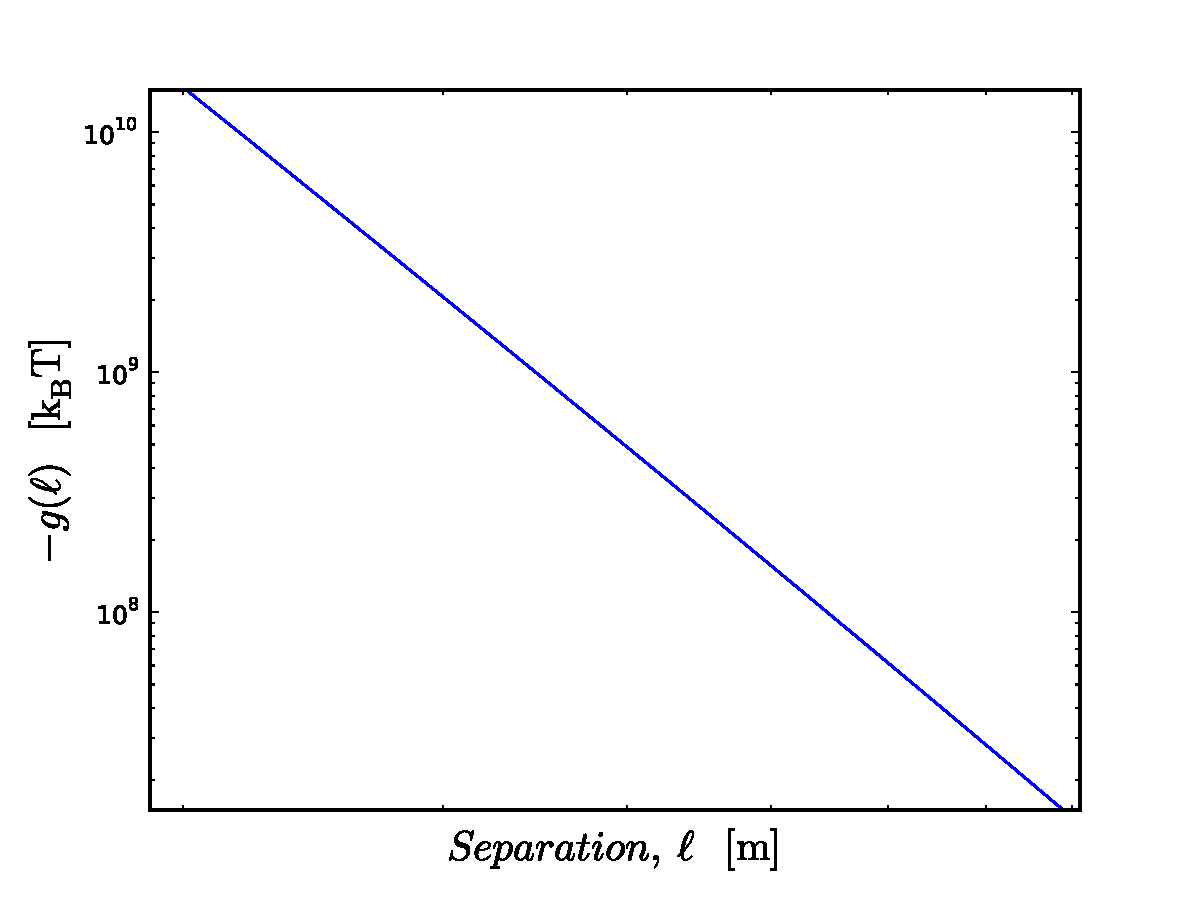
\includegraphics[width=8cm]{./140220_cyl-cyl/Full_parallel_g_vs_l.pdf}}
\caption{\label{full_par} Using equations \ref{retardedfinal-a} and \ref{retardedfinal-b}, Full result for parallel cylinders as a function of separation}
\end{figure}

We now again transform this result into a form that is suitable for computation and numerical implementation. Rewriting Eq. \ref{retardedfinal} as
\begin{equation}
  \fbox{
    $\displaystyle{
g(\ell) = - \frac{3 (\pi R_1^{2}) (\pi R_2^{2})}{8\pi~\ell^5} {\cal A}(\ell),}$}
\label{retardedfinal-a}
\end{equation}
we introduced the Hamaker coefficient
\begin{equation}
{\cal A}(\ell) = \frac{k_BT}{12 \pi} {\sum_{n=0}^{\infty}}' \Delta_{1,\parallel} \Delta_{2,\parallel} 
\int_{1}^{+\infty}\!\!\!\!\! \frac{dy}{\sqrt{y^2 - 1}} \int_0^{\infty}\!\!\!  u du ~\frac{e^{-2 y \sqrt{u^{2} + p_n^{2}(\ell)}}}{(u^{2} +p_n^{2}(\ell))^{1/2}} ~h(a_1(i \omega_n), a_2(i \omega_n), u, p_n^{2}(\ell))
\label{retardedfinal-b}
\end{equation}
with $h(a_1(i \omega_n), a_2(i \omega_n), u, p_n^{2}(\ell))$ defined in Eq. \ref{fcfenhjqwk}. This result is simpler then in the skewed case becasue it does not contain any angle dependence. In general ${\cal A}(\ell)$ can not be written in terms of ${\cal A}^{(0)}(\ell)$ and ${\cal A}^{(2)}(\ell)$ of the skewed cylinders.


\subsection{Parallel cylinders - non-retarded result}


In the non-retarded limit, $c \longrightarrow \infty$, the above formula  reduces to 
\begin{widetext}
\begin{eqnarray}
g(\ell; c \longrightarrow \infty) &=& - \frac{k_BT}{32} \frac{ R_1^{2} R_2^{2} }{\ell^5} {\sum_{n=0}^{\infty}}' \Delta_{1,\parallel} \Delta_{2,\parallel} 
\left( 3 + 5 (a_1+a_2) + 19 a_1 a_2 \right) \int_{1}^{+\infty}\!\!\!\!\! \frac{dy}{\sqrt{y^2 - 1}} \int_0^{\infty}\!\!\! u^4 du ~{e^{-2 y u }} = \nonumber\\
& & - \frac{9 ~k_BT}{(64 \times 32) \pi } \frac{\pi^2 R_1^{2} R_2^{2}}{\ell^5} {\sum_{n=0}^{\infty}}' \Delta_{1,\parallel} \Delta_{2,\parallel}
\left \{ 3 + 5 [ a_1(i \omega_n) + a_2(i \omega_n) ] + 19 a_1(i \omega_n) a_2(i \omega_n) \right \}.
\label{eq:cyl-paral-nonretarded}
\end{eqnarray}
\end{widetext}
Let us assume that the two cylinders are identical with radius $a$, so that we can finally write
\begin{equation}
  \fbox{
    $\displaystyle{
g(\ell; c \longrightarrow \infty) = - \frac{3}{(32^2) \pi } \frac{(\pi a^2)^{2}}{\ell^5} {\cal A}(\ell = 0),
\label{eq:cyl-paral-nonretarded-frq3}}$}
\end{equation}
where
\begin{equation}
{\cal A}(\ell = 0) = {\textstyle\frac32} {k_BT} ~ {\sum_{n=0}^{\infty}}' \Delta_{1,\parallel} \Delta_{2,\parallel}
\Big( 3 + 5 [ a_1(i \omega_n) + a_2(i \omega_n) ] + 19 a_1(i \omega_n) a_2(i \omega_n) \Big)
\label{eq:cyl-paral-nonretarded-frq3_A}
\end{equation}

%%%%%%%%%%%%%%%%%%%%%%%%%%%%%%%%%%%%%%%%%%%%%%%%%%%%%%%%%%%%%%%%%%%%%%%%%%%%%%%
%Par_nonret
\begin{figure}[t]
\centerline{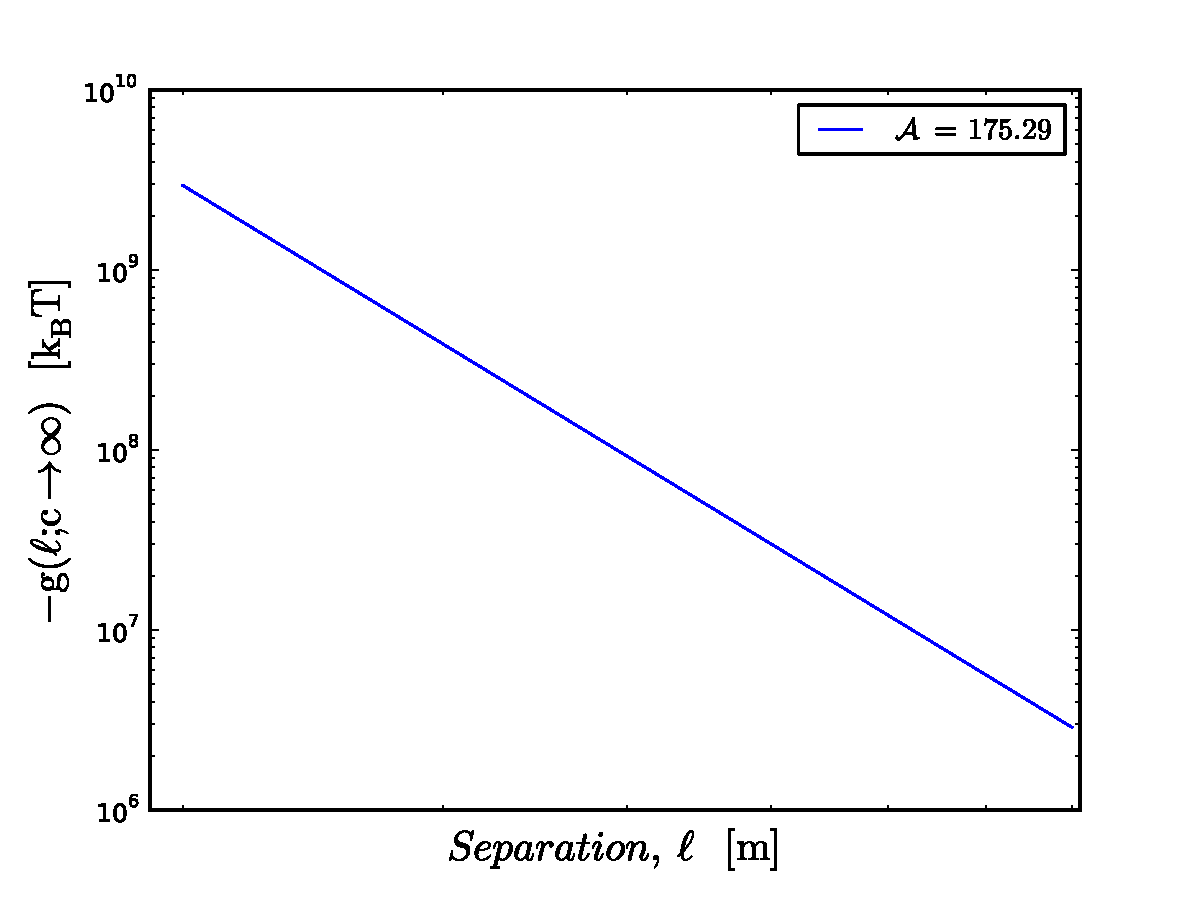
\includegraphics[width=8cm]{./140220_cyl-cyl/Nonret_parallel_G_vs_l.pdf}}
\caption{\label{f} Using equations \ref{eq:cyl-paral-nonretarded-frq3} and \ref{eq:cyl-paral-nonretarded-frq3_A}, non-retarded result for parallel cylinders as a function of separation, Eq. \ref{eq:cyl-paral-nonretarded-frq3_A} ${\cal A}(\ell = 0) = 175.29$.}
\end{figure}

For the case where the two interacting cylinders are composed of solid isotropic dielectric materials this form of the interaction free energy can be compared with the result obtained by Barash and Kyasov ( Eq. 10 in Ref. \onlinecite{Barash89}) and can be reduced to it {\sl exactly}. Again the $n = 0$ term of this formula for two identical cylinders corresponds to classical dipolar fluctuation forces as analyzed in Ref. \onlinecite{parscylinders}.

With definitions Eq. \ref{eq:adef}
\begin{equation}
a_{1,2}(i \omega_n) = \frac{2 \Delta_{\perp}^{(1,2)}(i \omega_n)}{\Delta_{\parallel}^{(1,2)}(i \omega_n)} = 2 \frac{({{\epsilon^{c}}_{\perp}}^{(1,2)}(i \omega_n) -\epsilon_{m}(i \omega_n)) \epsilon_{m}(i \omega_n)}{({{\epsilon^{c}}_{\perp}}^{(1,2)}(i \omega_n)+\epsilon_{m}(i \omega_n)) ({{\epsilon^{c}}_{\parallel}}^{(1,2)}(i \omega_n) -\epsilon_{m}(i \omega_n))}
\end{equation}
we then obtain
\begin{equation}
{\cal A}(\ell = 0) = {\textstyle\frac32} {k_BT} ~ {\sum_{n=0}^{\infty}}' \Big( 3~ \Delta_{1,\parallel} \Delta_{2,\parallel}
 + 10 [ \Delta_{\perp}^{(1)}\Delta_{2,\parallel} + \Delta_{\perp}^{(2)}\Delta_{1,\parallel} ] + 76~ \Delta_{\perp}^{(1)} \Delta_{\perp}^{(2)}\Big)
\end{equation}
This is exactly the same as obtained by Parsegian as cited in Ref. \cite{Parscyl}.

\section{Parallel cylinders - zero temperature result}

As with skewed cylinders, we can take the zero temperature limit where the summation over the Matsubara frequencies becomes an integral over $n$ with $dn = \hbar/(2\pi ~k_BT) d\omega$. Again we introduce $x = \frac{\ell}{c} \sqrt{t^2 + 1} ~\omega$. Then, as for skewed cylinders, we obtain the interaction free energy per unit length of two parallel cylinders,
\begin{widetext}
\begin{equation}
g(\ell) = -\frac{\hbar c}{64 \pi^3} \frac{\pi^2 R_1^{2} R_2^{2}}{\ell^6}  \epsilon_m(0)^{5/2} \Delta_{1,\parallel}(0) \Delta_{2,\parallel}(0) 
\!\! \int_0^{\infty} dx~ x^5 \int_{1}^{+\infty}\!\!\!\!\! \frac{dy}{\sqrt{y^2 - 1}} \int_0^{\infty} \frac{t dt ~e^{- 2 \sqrt{\epsilon_m(0)} ~y x}}{(t^2 + 1)^{7/2}} \tilde h(t, a_1(0), a_2(0)).
\end{equation}
\end{widetext}
Here 
\begin{widetext}
\begin{equation}
\tilde h(t, a_1, a_2) =   2 \left[ (1+3a_1)(1+3a_2) t^{4} + 2 (1+2a_1+2a_2+3a_1a_2) t^{2}  + 2(1+a_1)(1+a_2)\right] +  (1-a_1)(1-a_2)(t^{2} + 2)^2 .
\end{equation}
\end{widetext}
The spatial dependence is, again, one power higher in the retarded regime than in the non-retarded regime. All the frequency dependence of the material properties in the retarded limit is again reduced to the static response as in the Lifshitz analysis \cite{LL}.


\section{Screened zero frequency term}

Because of the presence of salt the zero frequency (classical) contribution to the Hamaker coefficients is screened. This means that instead of the Laplace equation one should take into account the linearized Debye-Huckel equation. This is of course approximate and more sophisticated statistical mechanical theories could be taken into account. Nevertheless we remain within the framework of the inearized Debye-Huckel theory.

Instead of going through the derivation once again for this case we note that within the DH approximation formally Eq. \ref{eq:d2f} would remain the same if we make the substitution $\epsilon_m \frac{\omega_n^{2}}{c^{2}} \longrightarrow \kappa^2$, where $\kappa^2$ is the inverse Debye screening length. This means that the $n=0$ term of Eq. \ref{pars-31} could be written as 
\begin{equation}
G^{(0)}(\ell,\theta) = - \frac{k_BT}{64 \times 2 \pi} \frac{ (\pi R_1^{2}) (\pi R_2^{2}) }{\ell^{4} \sin{\theta}} ~ \Delta_{1,\parallel} \Delta_{2,\parallel} ~(\kappa \ell)^{4} ~\int_0^{\infty} t dt ~\frac{e^{- 2 (\kappa \ell) \sqrt{t^{2} + 1}}}{(t^{2} + 1)} \tilde g(t, a_1(0), a_2(0), \theta),
\label{pars-31deqw }
\end{equation}
where we took into account that on the DH level $p_n^{2}(\ell) =  \epsilon_m(i \omega_n) \frac{\omega_n^{2}}{c^{2}} \ell^{2} \longrightarrow \kappa^2  \ell^{2} $ and everything else remains unchanged. 

Analogously the zero frequency term for the parallel cylinder case Eq. \ref{retardedfinal} would be modified to 
\begin{equation}
g^{(0)}(\ell) = - \frac{k_BT}{32\times 2 ~\pi^2} \frac{(\pi R_1^{2}) (\pi R_2^{2}) }{\ell^5} ~ \Delta_{1,\parallel} \Delta_{2,\parallel} 
\int_{1}^{+\infty}\!\!\!\!\! \frac{dy}{\sqrt{y^2 - 1}} \int_0^{\infty}\!\!\!  u du ~\frac{e^{-2 y \sqrt{u^{2} + (\kappa \ell)^{2}}}}{(u^{2} +(\kappa \ell)^{2})^{1/2}} ~h(a_1(0), a_2(0), u, (\kappa \ell)^{2}),
\label{retardedfinal-1}
\end{equation}
and
\begin{widetext}
\begin{eqnarray}
h(a_1(0), a_2(0), u, (\kappa \ell)^{2}) &=&   2 \left[ (1+3a_1)(1+3a_2) u^{4} + 2 (1+2a_1+2a_2+3a_1a_2) u^{2} (\kappa \ell)^{2} + 2(1+a_1)(1+a_2) (\kappa \ell)^{4}\right]  + \nonumber \\
& &  (1-a_1) (1-a_2) (u^{2} + 2 (\kappa \ell)^{2})^2 .
\label{fcfenhjqwk-1}
\end{eqnarray}
\end{widetext}
This completes the derivation of the van der Waals interactions between two anisotropic cylinders at all separations. On the lowets level one needs not take into account the above derivation fo the zero frequency term but just skip it in th efrequency summation. This would give correctly the vdW interactions at separations larger then the Debye length.

\section{Interactions at small spacings}

We take the main results from Ref. \cite{rick1}. In the limit of small separations between the two cylinders $\ell/a\longrightarrow0$,
we reformulate the approach based on the \emph{Derjaguin} \textsl{method}
and introduced for a single cylinder and a substrate. For closely
opposed curved surfaces where $c_{1}^{1},c_{2}^{1}$ are the principal
curvatures of the surface $1$ and $c_{1}^{2},c_{2}^{2}$ are the
principal curvatures of the surface $2$, the \emph{Derjaguin} \textsl{method}
leads to the interaction energy of the form \begin{equation}
G(\ell,\theta;a_{1},a_{2})=\int\int_{-\infty}^{+\infty}{\cal G}(\ell+{\textstyle \frac{1}{2}}c_{1}x^{2}+{\textstyle \frac{1}{2}}c_{2}y^{2})~dxdy,\label{equ78}\end{equation}
 where $c_{1}$ and $c_{2}$ are defined as \begin{equation}
c_{1}c_{2}=(c_{1}^{1}c_{2}^{1}+c_{1}^{2}c_{2}^{2})+(c_{1}^{1}c_{1}^{2}+c_{2}^{1}c_{2}^{2})\sin^{2}{\theta}+(c_{1}^{1}c_{2}^{2}+c_{1}^{1}c_{2}^{2})\cos^{2}{\theta}.\end{equation}
 With polar variables the integral Eq. \ref{equ78} can be rewritten
as \begin{equation}
G(\ell,\theta;a_{1},a_{2})=\int_{0}^{2\pi}\int_{0}^{+\infty}{\cal G}(\ell+{\textstyle \frac{1}{2}}\rho^{2})~\frac{\rho d\rho~d\phi}{\sqrt{c_{1}c_{2}}}.\end{equation}
 For two cylinders with radii $a_{1}$ and $a_{2}$ at an angle $\theta$
the above equations can be cast in the form \begin{equation}
G(\ell,\theta;a_{1},a_{2})=\frac{2\pi\sqrt{a_{1}a_{2}}}{\sin{\theta}}\int_{\ell}^{{\infty}}{\cal G}(h,\theta)dh.\end{equation}
 This gives to the lowest order in the $\Delta$'s \begin{eqnarray}
G(\ell,\theta;a_{1},a_{2})=-\frac{\sqrt{a_{1}a_{2}}~k_{B}T}{8\pi~\ell~\sin{\theta}}{\sum_{n=0}^{\infty}}'\int_{0}^{2\pi}d\psi~{\Delta_{{\cal L}m}(\psi)\Delta_{{\cal R}m}(\theta-\psi)}.\end{eqnarray}
 The angular
integral is again analytically solvable for any anisotropy and leads
to the following result for the interaction free energy of two cylinders
of equal radii $a_{1}=a_{2}=a$ \begin{equation}
G(\ell,\theta;a)=-\frac{a~k_{B}T}{4~\ell~\sin{\theta}}\left({\cal H}^{(0)}+{\cal H}^{(2)}\cos^{2}{\theta}\right),\end{equation}
 where ${\cal H}^{(0)}$ and ${\cal H}^{(2)}$ are obtained from \begin{equation}
{\cal H}^{(0)}+~{\cal H}^{(2)}=\frac{1}{2\pi}{\sum_{n=0}^{\infty}}'\int_{0}^{2\pi}d\psi\left(\frac{{{\epsilon^{c}}_{\perp}({\cal R})}\sqrt{1+{\gamma^{c}}({\cal R})\cos^{2}{\psi}}-\epsilon_{m}}{{{\epsilon^{c}}_{\perp}({\cal R})}\sqrt{1+{\gamma^{c}}({\cal R})\cos^{2}{\psi}}+\epsilon_{m}}\right)\left(\frac{{{\epsilon^{c}}_{\perp}({\cal L})}\sqrt{1+{\gamma^{c}}({\cal L})\cos^{2}{\psi}}-\epsilon_{m}}{{{\epsilon^{c}}_{\perp}({\cal L})}\sqrt{1+{\gamma^{c}}({\cal L})\cos^{2}{\psi}}+\epsilon_{m}}\right)\label{sutu11}\end{equation}
 and \begin{equation}
{\cal H}^{(0)}=\frac{1}{2\pi}{\sum_{n=0}^{\infty}}'\int_{0}^{2\pi}d\psi\left(\frac{{{\epsilon^{c}}_{\perp}({\cal R})}\sqrt{1+{\gamma^{c}}({\cal R})\cos^{2}{\psi}}-\epsilon_{m}}{{{\epsilon^{c}}_{\perp}({\cal R})}\sqrt{1+{\gamma^{c}}({\cal R})\cos^{2}{\psi}}+\epsilon_{m}}\right)\left(\frac{{{\epsilon^{c}}_{\perp}({\cal L})}\sqrt{1+{\gamma^{c}}({\cal L})\sin^{2}{\psi}}-\epsilon_{m}}{{{\epsilon^{c}}_{\perp}({\cal L})}\sqrt{1+{\gamma^{c}}({\cal L})\sin^{2}{\psi}}+\epsilon_{m}}\right).\label{sutu22}\end{equation}
 For two identical cylinders the ${\cal L}$ and ${\cal R}$ values
are the same. Again we omit writing the explicit frequency dependence
of all the dielectric functions. This dependence should be entered
when numerical calculations are performed. Here again \begin{equation}
{\gamma^{c}}=\frac{{{\epsilon^{c}}_{\parallel}}-{{\epsilon^{c}}_{\perp}}}{{{\epsilon^{c}}_{\perp}}},
\end{equation}
 and ${\epsilon^{c}}_{\perp}$ and ${\epsilon^{c}}_{\parallel}$ are
the transverse and longitudinal dielectric responses of the cylinder
and $\epsilon_{m}$ that of the solution medium.

As above we now introduce the Hamaker coefficients
according to the definitions \begin{equation}
{\cal A}^{(0)}={\textstyle \frac{3}{2}}k_{B}T~{\cal H}^{(0)}\qquad{\rm and}\qquad{\cal A}^{(2)}={\textstyle \frac{3}{2}}k_{B}T~{\cal H}^{(2)},\end{equation}
 and thus obtain for the interaction free energy of the two cylinders
of equal radii $a_{1}=a_{2}=a$ \begin{equation}
 \fbox{
    $\displaystyle{
G(\ell,\theta;a)=-\frac{a}{6~(\ell - 2a)~\sin{\theta}}\left({\cal A}^{(0)}+{\cal A}^{(2)}\cos^{2}{\theta}\right).}$}\end{equation}
 This is the final expression for the interaction free energy
between two cylinders at a general angle $\theta$ and separation $\ell$
in the proximal limit. 

Examine now the interaction free energy of two identical anisotropic
cylinders of radius $a$ at zero mutual angle. In this case the interaction free
energy \textbf{per unit length} can be obtained in the form 
(\cite{Parsegian}, p.172)
\begin{equation}
g(\ell,\theta;a)=-\frac{k_{B}T \sqrt{a}}{16~\ell^{3/2}}~\left({\cal H}^{(0)}+{\cal H}^{(2)}\right),\label{pop-equ25}\end{equation}
 where ${\cal H}^{(0)}$ and ${\cal H}^{(2)}$ are obtained in complete
analogy to Eq. \ref{sutu11} and \ref{sutu22} from \begin{equation}
{\cal H}^{(0)}+~{\cal H}^{(2)}=\frac{1}{2\pi}{\sum_{n=0}^{\infty}}'\int_{0}^{2\pi}d\psi\left(\frac{{{\epsilon^{c}}_{\perp}({\cal R})}\sqrt{1+{\gamma^{c}}({\cal R})\cos^{2}{\psi}}-\epsilon_{m}}{{{\epsilon^{c}}_{\perp}({\cal R})}\sqrt{1+{\gamma^{c}}({\cal R})\cos^{2}{\psi}}+\epsilon_{m}}\right)\left(\frac{{{\epsilon^{c}}_{\perp}({\cal L})}\sqrt{1+{\gamma^{c}}({\cal L})\cos^{2}{\psi}}-\epsilon_{m}}{{{\epsilon^{c}}_{\perp}({\cal L})}\sqrt{1+{\gamma^{c}}({\cal L})\cos^{2}{\psi}}+\epsilon_{m}}\right).\label{pop-stu11}\end{equation}
 Of course, for two identical cylinders, the $\epsilon$ values for ${\cal L}$ and ${\cal R}$ are the same. Introducing again the Hamaker coefficient as before 
\begin{equation}
\left({\cal A}^{(0)}+{\cal A}^{(2)}\right)={\textstyle \frac{3}{2}}k_{B}T~\left({\cal H}^{(0)}+{\cal H}^{(2)}\right),\end{equation}
we get the interaction free energy per unit length of the parallel cylinders expressed throug the surface to surface separation
 \begin{equation}
  \fbox{
    $\displaystyle{
g(\ell,a)=-\frac{\sqrt{a}}{24~(\ell - 2a)^{3/2}}~\left({\cal A}^{(0)}+{\cal A}^{(2)}\right).\label{pop-equ26}}$}
\end{equation}
 This is now the sixth and last result that we will use to quantify
the van der Waals - London dispersion interaction between two parallel
cylindrical CNTs at small separations. 

\subsection{Grosberg's interpolation formula}

Let us now compare Eq. \ref{eq:cyl-paral-nonretarded-frq3} and Eq. \ref{pop-equ26} for two equal cylinders of radius $a$. We have 
\begin{equation}
g(\ell) = - \frac{3}{(32^2) \pi } \frac{(\pi a^2)^{2}}{\ell^5} {\cal A}(\ell = 0), \qquad g(\ell)=-\frac{\sqrt{a}}{24~(\ell - 2a)^{3/2}}~\left({\cal A}^{(0)}+{\cal A}^{(2)}\right).
\end{equation}
Grosberg \cite{Grosb} showed that there is an interpolation formula for
\begin{equation}
\frac{g(\ell,a) \ell}{\beta^2} = \left\{ 
\begin{array}{cc}
\left( \frac{\beta \pi}{4}\right)^2 &; \beta \ll 1\\ ~ & ~ \\
\left( \frac{\pi}{576}\right) \left( 1 - 2 \beta\right)^{-3/2} &;  1 - 2 \beta \ll 1 \\
\end{array}
\right.
\end{equation}
with $\beta = a/\ell$, of the form
\begin{equation}
\frac{g(\ell,a) \ell}{\beta^2} = \left( \frac{\beta \pi}{4}\right)^2 \left( 1 - 2 \beta\right)^{-3/2} \left( 1 - 2 \beta + \frac{2 \beta}{9 \pi} \right)
\end{equation}
Our formulas are however not of the Hamaker-type that Grosberg was using, so the Hamaker coefficient for the small and large separation limit are not the same. In our case we have rather
\begin{equation}
\frac{g(\ell,a) \ell}{\beta^2} = \left\{ 
\begin{array}{cc}
\frac{3 \pi}{32^2} {\cal A}(\ell = 0) ~\beta^2 &; \beta \ll 1\\ ~ & ~ \\
\frac{1}{6 \sqrt2} \left({\cal A}^{(0)}+{\cal A}^{(2)}\right) ~\left( 1 - 2 \beta\right)^{-3/2} &;  1 - 2 \beta \ll 1 \\
\end{array}
\right.
\end{equation}

Nevertheless one can still use the same philosophy to derive
\begin{equation}
\frac{g(\ell,a) \ell}{\beta^2} = \frac{3 \pi}{32^2} {\cal A}(\ell = 0) ~\beta^2  \left( 1 - 2 \beta\right)^{-3/2} \left( 1 - 2 \beta + {\cal R} \frac{32^2 }{18 \sqrt2 \pi} ~ (2 \beta) \right)
\end{equation}
where $\cal R$ is the ratio
\begin{equation}
{\cal R} = \frac{{\cal A}^{(0)}+{\cal A}^{(2)}}{{\cal A}(\ell = 0)}.
\end{equation}
This should be used as an interpolation formula between the small and the large separation regimes. This can be written also as
\begin{equation}
g(\ell,a) = g_{>}(\ell,a) \left( 1 - 2 \beta\right)^{-1/2} + {32~ \beta^5} g_{<}(\ell,a),
\end{equation}
where $g_{>}(\ell,a)$ is the interaction free energy per unit length at large separations, $\beta \ll 1$, that goes into the non-retarded form still at large separations and $g_{<}(\ell,a) $ is the non-retarded (of course) interaction free energy at small separations $1- 2\beta \ll 1$. This seems to complete the analysis.


\begin{thebibliography}{99}

\bibitem{dressel} R. Saito, G. Dresselhaus and M. S. Dresselhaus, {\sl Physical Properties of Carbon Nanotubes} (World Scientific Publishing Company; 1st edition) (1998).
\bibitem{rick1} R. F. Rajter, R. H. French, R. Podgornik, W. Y. Ching, and V. A. Parsegian, {\sl J Appl Phys} {\bf 104} 053513 (2008).
\bibitem{capasso-IEEE} F. Capasso, J. N. Munday, D. Iannuzzi and H. B. Chan, {\sl IEEE Journal of Selected Topics in Quantum Electronics} {\bf 13} 400 (2007). 
\bibitem{otherwork} D.J. Mitchell, B.W. Ninham and P. Richmond, {\sl Biophys. J.} {\bf 13} 359 (1973).  G Barton, {\sl J. Phys. A: Math. Gen.} {\bf 34} 4083 (2001). S. J. Rahi, A. W. Rodriguez, T. Emig, R. L. Jaffe, S. G. Johnson, and M. Kardar, {\sl Phys. Rev. A } {\bf 77} 030101 (RC)  (2008). S. J. Rahi, T. Emig, R. L. Jaffe, M. Kardar, {\sl Phys. Rev. A} {\bf 78} 012104 (2008).  
\bibitem{rick2} R. F. Rajter, R. Podgornik, V. A. Parsegian, R. H. French, and W. Y. Ching, {\sl Phys Rev B} {\bf 76} 045417 (2007). 
\bibitem{Barash} Yu. S. Barash, {\sl Izv. Vyssh. Uchebn. Zaved. Radiofiz.} {\bf 21} 163 (1978). J. N. Munday, D. Iannuzzi, Yu. S. Barash and F. Capasso, {\sl Phys. Rev. A} {\bf 71} 042102 (2005). Both papers contain a typo that was amended in \cite{erratum}.
\bibitem{erratum} J. N. Munday, D. Iannuzzi, Yu. Barash and F. Capasso, {\sl Phys. Rev. A} {\bf 78} 029906 (2008). (Erratum) 
\bibitem{Parsegian} V. A. Parsegian, \textsl{Van der Waals Forces}, Cambridge University Press, Cambridge (2005). 
\bibitem{Ninham}  J. Mahanty and B.W. Ninham, {\sl Dispersion Forces}, (Academic Press, London, 1976).
\bibitem{Pitaevskii} L. P. Pitaevskii, {\sl Sov. Phys. JETP} {\bf 10} 408 (1960).
\bibitem{Barash89} Yu. S. Barash and A.A. Kyasov, {\sl Sov. Phys. JETP} {\bf 68} 39 (1989).
\bibitem{philbin} T.G. Philbin, U. Leonhardt, {\sl Phys. Rev. A} {\bf 78} 042107 (2008). 
\bibitem{parscylinders} V.A. Parsegian, {\sl J. Chem. Phys.}  {\bf 56} 4393 (1972). R. Podgornik and V. A. Parsegian, {\sl Phys. Rev. Letts.} {\bf 80} 1560 (1998). 
\bibitem{LL} L. D. Landau, E. M. Lifshitz, L. P. Pitaevskii, {\sl Statistical Physics: Volume 9}. (Butterworth-Heinemann, 1980), pp. 341-345.
\bibitem{Abel} R. N. Bracewell, The  Fourier Transform and Its Applications (McGraw–Hill, New York, 1986).
\bibitem{Mintmire_CNT_overview} C. T. White, J. W. Mintmire, {\sl J. Phys. Chem. B} {\bf 109} 2 (2005). 
\bibitem{Rajter_e2_LD} R. F. Rajter, PhD thesis, MIT (2009).
%\bibitem{Samsonidze}   Ge. G. Samsonidze, R. Saito, N. Kobayashi, A. Gruneis, J. Jiang,  A. Jorio, S. G. Chou, G. Dresselhaus, and M. S. Dresselhaus, {\sl Appl. Phys. Lett.} {\bf 85} 5703 (2004).
\bibitem{Elbaum} M. Elbaum and M. Schick, {\sl Phys. Rev. Lett.} {\bf 66} 1713 (1991)
\bibitem{DLP1959} I.E. Dzyaloshinskii, E.M. Lifshitz and L.P. Pitaevskii, {\sl Adv. Phys.} {\bf 10} 165 (1959).
\bibitem{ParsegianNature} J.N. Munday, F. Capasso, and V.A. Parsegian, {\sl Nature} {\bf 457} 170 (2009).
\bibitem{rick1} 
Rick F. Rajter, Rudi Podgornik, V. Adrian Parsegian, Roger H. French, and W. Y. Ching, PHYSICAL REVIEW B {\bf 76} 045417 (2007).
\bibitem{Parscyl}
R. Podgornik and V. A. Parsegian, Phys. Rev. Letts. {\rm 80} 1560 (1998).
\bibitem{Grosb}
A. Yu. Grosberg,  Biofizika  {\bf 5} 913 (197?).

\end{thebibliography}

\end{document}
